\documentclass[10pt, a4paper]{article}
\usepackage[utf8]{inputenc}
\usepackage[frenchb]{babel}
\usepackage[OT1]{fontenc}
\usepackage{amsfonts, amsmath, amssymb, amsthm, dsfont, amsthm}
\usepackage{a4wide}
\usepackage[dvipsnames]{xcolor}
\usepackage{tikz} 
\usetikzlibrary{arrows,positioning,shapes}

\title{\textbf{Lab Report} \\ Week of 12/01/2016}
%\author{Olivier \textsc{Mangin}}
%\date{\today}

\definecolor{main}{named}{BurntOrange}
\definecolor{second}{named}{RoyalBlue}
%\newcommand{\maincolor}{orange}
%\newcommand{\secondcolor}{orange!20}
\newcommand{\strong}[1]{\textcolor{main}{\textbf{#1}}}
\newcommand{\stronger}[1]{\textcolor{second}{\textbf{#1}}}
\newcommand{\colored}[1]{\textcolor{main}{#1}}

% Affichage du titre avec les numéro et date de la semaine
\newcommand{\titre}[2]{
\noindent
\hspace{-10pt}
\begin{tabular}{lr}
  \hspace{0.58\textwidth} & \hspace{0.4\textwidth} \\
  \strong{\huge Lab Report} & \textbf{\Large #1} \medskip \\
  \textbf{\Large Name \& Roll} & {\large #2} ~\\
\end{tabular}

\vspace{20pt}
}

% Encadré ``En bref'' réumant les avancées et problèmes de la semaine
\newenvironment{enbref}{
\noindent\fcolorbox{main}{main}{
\begin{minipage}{\textwidth}
\textcolor{white}{\textbf{\large }}
\end{minipage}
} \\

}{
\begin{center}
  \strong{ \rule[2mm]{\textwidth}{3pt} }
\end{center}
\vspace*{-20pt}
}

% Affichage d'un titre de rubrique
\newcommand{\rubrique}[1]{
  \bigskip
  \begin{center}
  \begin{minipage}{\textwidth}
    \noindent\strong{{\large #1} \\
      \rule[2mm]{\textwidth}{1pt} }
  \end{minipage}
  \end{center}
  \vspace*{-20pt}
}

% Symbole utilisé en début de ligne des éléments
\newcommand{\doublerect}{
\begin{tikzpicture}
  \fill[color=main] (0,0) rectangle (4pt,-4pt);
  \fill[color=second] (2pt,-2pt) rectangle (6pt,-6pt);
\end{tikzpicture}
}

% Affichage d'un titre d'élément
\newcommand{\element}[1]{
  \medskip
  \noindent\textcolor{second}{ \doublerect \textbf{#1}}
}

% Pour les lectures, petit raccourci pour mettre en avant le niveau
% de lecture d'un article.
\newcommand{\lu}{\strong{[Lu]} }
\newcommand{\parcouru}{\strong{[Parcouru]} }
\newcommand{\alire}{\strong{[A lire]} }
\newcommand{\presentation}{\strong{[Présentation]} }
\newcommand{\keynote}{\strong{[Keynote]} }



\usepackage[pdfauthor={Name}, pdftitle={Weekly}, pdfsubject={Week 1}, pdfkeywords={},colorlinks=true,urlcolor=black,linkcolor=black, citecolor=black]{hyperref}
\usepackage{listings}
\usepackage{subfig}
\usepackage{graphicx}
\lstset{%
language=Matlab,
frame=single,
%numbers=left,
%numberstyle=\footnotesize,
%tabsize=2,
keepspaces=true,
columns=fullflexible,
basicstyle=\ttfamily\scriptsize,
keywordstyle=\color{blue}
}


\begin{document}

\renewcommand{\labelitemi}{\textcolor{main}{\small $\blacktriangleright$}}
\renewcommand{\labelitemii}{\textcolor{second}{\scriptsize \textbullet}}

\titre{Week 4}{09/02/2017}

\begin{enbref}
\element{Title}
\begin{itemize}
\item Choose any primitive and apply all basic 2D transformations
1). OpenGL
2). MatLab
\end{itemize}
\medskip

%\element{Problèmes rencontrés}
%\begin{itemize}
%\item Néant.
%\end{itemize}
\end{enbref}

%\rubrique{Lectures}
%Néant.
%\element{\lu ... \cite{...}}

\rubrique{Procedure}
\vspace{0.5mm} \flushleft

\element {OpenGL}

\vspace{0.5mm} \flushleft
1). Choose any primitive and apply all basic 2D transformations.
\begin{itemize}
\item Create a C file and name it as \textit{transformations.c}.

\item Following is the final code for all basic 2D transformations : 
\begin{lstlisting}
#include <stdio.h>
#include <math.h>
#include <GL/glut.h>
#include <stdlib.h>
#define PI 3.14159265
int flag, count; int i = 0 ; int j = 0 ; int k = 0 ;
double input_pts[10][2];
double final_pts[10][2];
double trans_matrix[3][3];

double x = 0 ;

void displayPolygon()
{

        glClear(GL_COLOR_BUFFER_BIT);
        glLineWidth(3);
        glBegin(GL_LINES);
                glColor3f(1.0f, 1.0f, 1.0f);
                glVertex2f(0.0f,400.0f);
                glVertex2f(0.0f,-400.0f);
                glVertex2f(400.0f,0.0f);
                glVertex2f(-400.0f,0.0f);
        glEnd();

        glBegin(GL_LINE_LOOP);

        glColor3f(1.0f,0.0f,0.0f);

        glVertex3f(input_pts[0][0]/100.0, input_pts[0][1]/100.0, 1.0f);
        glVertex3f(input_pts[1][0]/100.0, input_pts[1][1]/100.0, 1.0f);
        glVertex3f(input_pts[2][0]/100.0, input_pts[2][1]/100.0, 1.0f);
        glVertex3f(input_pts[3][0]/100.0, input_pts[3][1]/100.0, 1.0f);
        glEnd();

        glBegin(GL_LINE_LOOP);

        glColor3f(0.0f,1.0f,0.0f);
        glVertex3f(final_pts[0][0]/100.0, final_pts[0][1]/100.0, 1.0f);
        glVertex3f(final_pts[1][0]/100.0, final_pts[1][1]/100.0, 1.0f);
        glVertex3f(final_pts[2][0]/100.0, final_pts[2][1]/100.0, 1.0f);
        glVertex3f(final_pts[3][0]/100.0, final_pts[3][1]/100.0, 1.0f);
        glEnd();

	glFlush();
	glutSwapBuffers();
}

void matrix_multiplication()
{
        int i = 0 , j = 0 , k = 0 ;
        double a = 0 ; double b = 0 ;

        for(i = 0 ; i < 4 ; i++)
        {
                a = trans_matrix[0][0]*input_pts[i][0] + trans_matrix[0][1]*input_pts[i][1] + trans_matrix[0][2];
                b = trans_matrix[1][0]*input_pts[i][0] + trans_matrix[1][1]*input_pts[i][1] + trans_matrix[1][2];

                final_pts[i][0]=a;
                final_pts[i][1]=b;
        }
}


void translate(double x , double y)
{
	trans_matrix[0][0] = 1;
    	trans_matrix[0][1] = 0;
    	trans_matrix[0][2] = x;
    	trans_matrix[1][0] = 0;
    	trans_matrix[1][1] = 1;
    	trans_matrix[1][2] = y;
    	trans_matrix[2][0] = 0;
    	trans_matrix[2][1] = 0;
    	trans_matrix[2][2] = 1;
}

void scale_x_y(double sx, double sy) 
{
    	trans_matrix[0][0] = sx;
    	trans_matrix[0][1] = 0;
    	trans_matrix[0][2] = 0;
    	trans_matrix[1][0] = 0;
    	trans_matrix[1][1] = sy;
    	trans_matrix[1][2] = 0;
    	trans_matrix[2][0] = 0;
    	trans_matrix[2][1] = 0;
    	trans_matrix[2][2] = 1;
}

void reflectAroundX(void) 
{
    	trans_matrix[0][0] = 1;
    	trans_matrix[0][1] = 0;
    	trans_matrix[0][2] = 0;
    	trans_matrix[1][0] = 0;
    	trans_matrix[1][1] = -1;
    	trans_matrix[1][2] = 0;
    	trans_matrix[2][0] = 0;
    	trans_matrix[2][1] = 0;
    	trans_matrix[2][2] = 1;
}


void shearaboutY(double b) 
{
    	trans_matrix[0][0] = 1;
    	trans_matrix[0][1] = 0;
    	trans_matrix[0][2] = 0;
    	trans_matrix[1][0] = b;
    	trans_matrix[1][1] = 1;
    	trans_matrix[1][2] = 0;
    	trans_matrix[2][0] = 0;
    	trans_matrix[2][1] = 0;
    	trans_matrix[2][2] = 1;
}

void rotate(double a) 
{
	x = PI / 180 ;
	a = a*x;
    	trans_matrix[0][0] = cos(a);
    	trans_matrix[0][1] = -1 * sin(a);
    	trans_matrix[0][2] = 0;
    	trans_matrix[1][0] = sin(a);
    	trans_matrix[1][1] = cos(a);
    	trans_matrix[1][2] = 0;
    	trans_matrix[2][0] = 0;
    	trans_matrix[2][1] = 0;
    	trans_matrix[2][2] = 1;
}

void transformPoints()
{
        int choice ;
        printf("\nEnter your choice:\n1. Translation\n2. Scaling\n3. Reflection\n4. Shear\n5. Rotate\n");
        printf("Your choice : ");
        scanf("%d",&choice);

        double x , y , scale_factor_x, scale_factor_y, shear_factor ,rotation_angle ;

        if(choice==1) 
        {
                printf("Enter translate_x : ");
                scanf("%lf",&x);
                printf("Enter translate_y : ");
                scanf("%lf",&y);
                translate(x,y);
        }

        if(choice==2)
        {
                printf("Enter scale_factor_x : ");
                scanf("%lf",&scale_factor_x);
                printf("Enter scale_factor_y : ");
                scanf("%lf",&scale_factor_y);
                scale_x_y(scale_factor_x,scale_factor_y);
        }

        if(choice==3)
        {
                reflectAroundX();
        }

        if(choice==4)
        {
                printf("\nEnter  the shearing Factor :  ");
                scanf("%lf",&shear_factor);
                shearaboutY(shear_factor);
        }

        if(choice==5)
        {
                printf("\nEnter the rotation_angle :  ");
                scanf("%lf",&rotation_angle);
                rotate(rotation_angle);
        }
}


int main(int argc, char **argv)
{
	glutInit(&argc, argv);
    	glutInitDisplayMode(GLUT_RGB);
    	glutInitWindowSize(800, 800);
    	for(i = 0 ; i < 10 ; i++)
        {
                for(j = 0 ; j < 3 ; j++)
                {
                        input_pts[i][j]=0;
                }
        }
    	printf("**********\nWe'll be applying  transformations to a sqaure polygon\n**********\n");
    	printf("Enter the polygon coordinates : ");
    	count = 4 ;

    	for( i = 0 ; i < count ; i++)
    	{
    		scanf("%lf %lf",&input_pts[i][0],&input_pts[i][1]);
    	}

        
        for(i = 0 ; i < 10 ; i++)
        {
                for(j = 0 ; j < 2 ; j++)
                {
                        final_pts[i][j]=0;
                }
        }
        for(i = 0 ; i < 3 ; i++)
        {
                for(j = 0 ; j < 3 ; j++)
                {
                        trans_matrix[i][j]=0;
                }
        }
    
    	transformPoints();
    	matrix_multiplication();
    	glClearColor(1.0, 1.0, 1.0, 1.0);
    	gluOrtho2D(-400, 400, -400, 400);
        glutCreateWindow("\nPolygon transformations");
        glutDisplayFunc(displayPolygon);
        glutMainLoop();

	return 0;
}

\end{lstlisting}

\vspace{0.5mm}

\item Compile and run the executable file in terminal by typing in the following commands : \\

\vspace{0.5mm} \flushleft

\textit{(a)\hspace{2mm} gcc transformations.c -lGL -lGLU -lglut -lm} \\
\textit{(b)\hspace{2mm} ./a.out}
\vspace*{1\baselineskip} 
\end{itemize}

\element {MatLab}\\

1). Choose any primitive and apply all basic 2D transformations

\begin{itemize}

\item Open a new Script and contruct a function transformations().
\item Following is the Matlab Script Code for all basic 2D transformations.
\begin{lstlisting}

function [] = transformations()
	disp("**************************************************************************")
	
	input_matrix = [0 0 1; 0 10 1; 10 10 1; 10 0 1 ; 0 0 1];
	disp("\nEnter your choice:\n1. Translation\n2. Scaling\n3. ReflectAroundX\n4. ShearaboutY\n5. Rotate\n");
	choice = input("Your choice : ");
	
	temp_matrix = [1 0 0; 0 1 0 ; 0 0 1];
	identity_matrix = [1 0 0; 0 1 0 ; 0 0 1];

	if(choice <= 5)
		if(choice==1)
			translate_x = input('Enter translate_x : ');
            		translate_y = input('Enter translate_y : ');
            		temp_matrix = [1 0 translate_x ; 0 1 translate_y ; 0 0 1];
		end

		if(choice==2)
			scale_factor_x = input('Enter scale_factor_x : ');
            		scale_factor_y = input('Enter scale_factor_y : ');
            		temp_matrix = [scale_factor_x 0 0 ; 0 scale_factor_y 0 ; 0 0 1];
            	end

            	if(choice==3)
            		temp_matrix = [1 0 0 ; 0 -1 0 ; 0 0 1];
            	end

            	if(choice==4)
            		shear_factor = input('Enter the shearing factor : ');
            		temp_matrix = [1 0 0 ; shear_factor 1 0 ; 0 0 1];
            	end

            	if(choice==5)
            		theta= input('Enter the rotation_angle : ');
            		theta = (theta*3.14159265) / 180 ;
			%theta = theta*_x;
            		temp_matrix = [cos(theta) -sin(theta) 0;
            				sin(theta) cos(theta) 0;
            				0 0 1];
            	end
        else
        	disp("\nYou choosed an invalid choice\n")
	end

	 

 	trans = transpose(temp_matrix);
 	final = input_matrix*trans;
      plot(input_matrix(:,1),input_matrix(:,2),'--','LineWidth', 3);
      hold on
      plot(final(:,1),final(:,2),'b-','LineWidth', 3);
\end{lstlisting}
\end{itemize}

\rubrique{Output}

\begin{figure}[ht!]
\centering
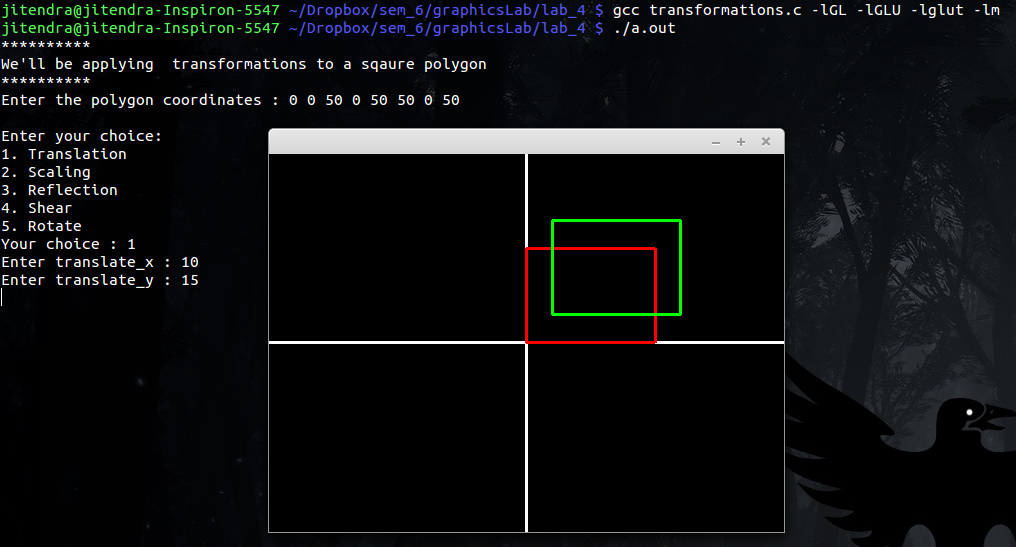
\includegraphics[width=60mm, height=60mm]{translationOpenGL.png}
\caption{translation in OpenGL \label{overflow}}
\end{figure}
\begin{figure}[ht!]
\centering
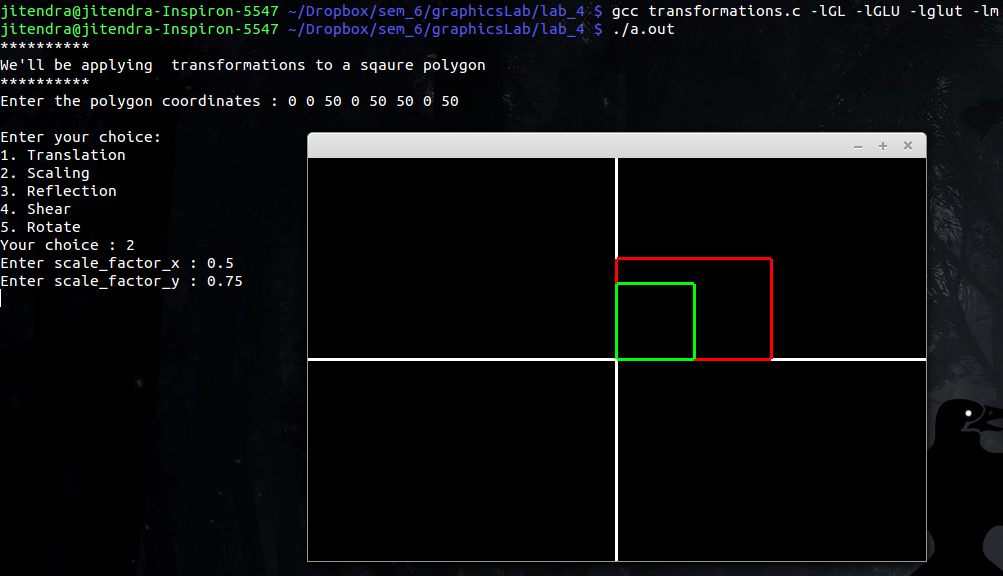
\includegraphics[width=60mm, height=60mm]{scalingOpenGL.png}
\caption{Scaling in OpenGL \label{overflow}}
\end{figure}
\begin{figure}[ht!]
\centering
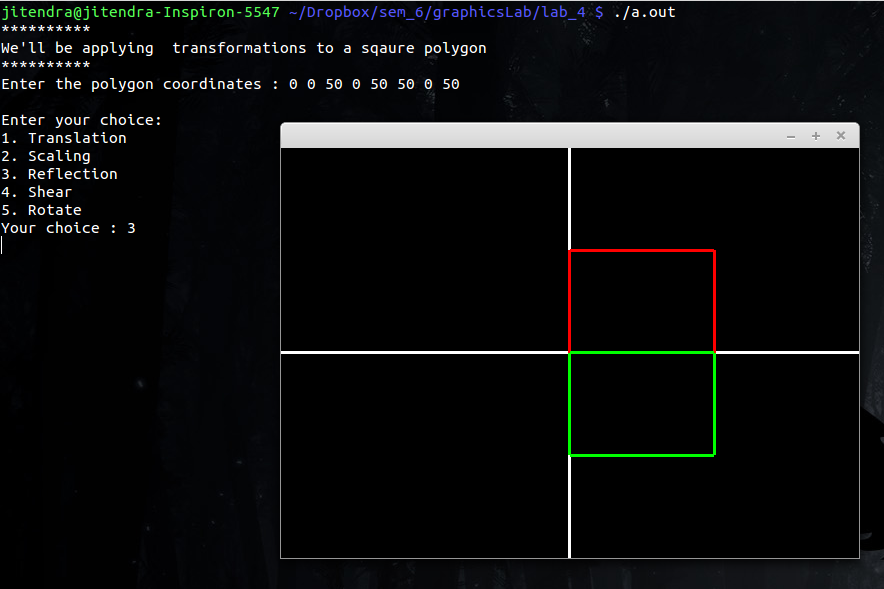
\includegraphics[width=60mm, height=60mm]{reflectionOpenGL.png}
\caption{reflection in OpenGL \label{overflow}}
\end{figure}
\begin{figure}[ht!]
\centering
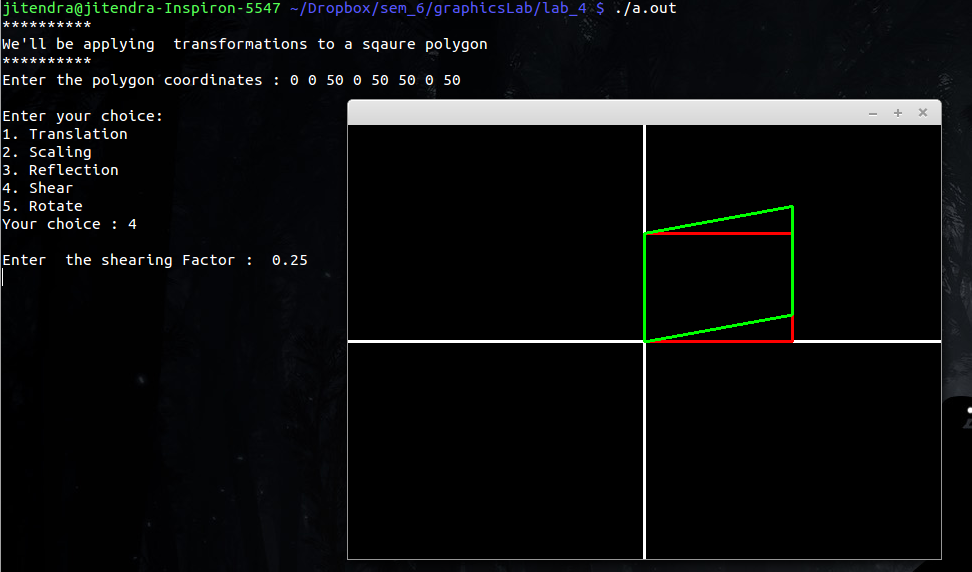
\includegraphics[width=60mm, height=60mm]{shearOpenGL.png}
\caption{Shear in OpenGL \label{overflow}}
\end{figure}
\begin{figure}[ht!]
\centering
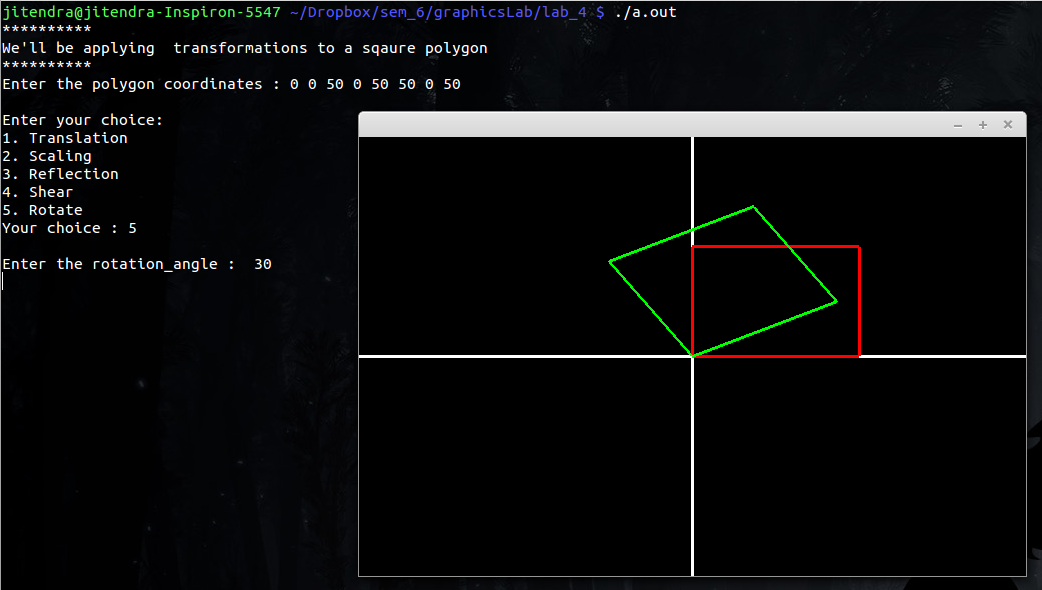
\includegraphics[width=60mm, height=60mm]{rotationOpenGL.png}
\caption{rotation in openGL \label{overflow}}
\end{figure}
\begin{figure}[ht!]
\centering
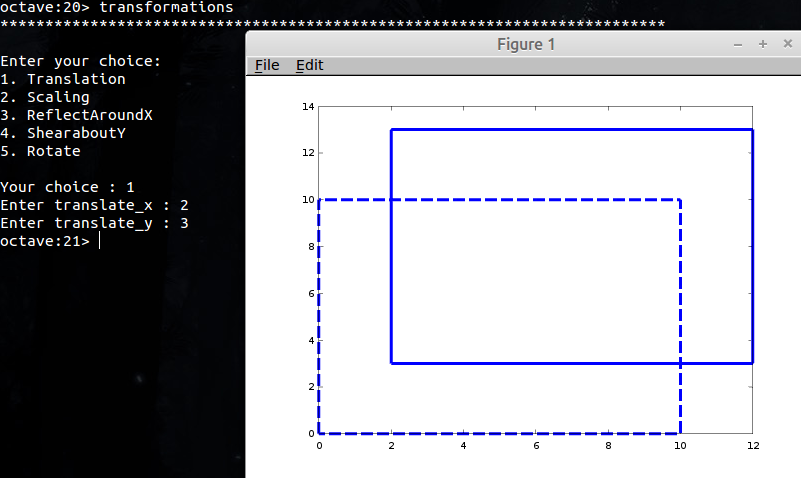
\includegraphics[width=60mm, height=60mm]{translationMatlab.png}
\caption{translation in matlab \label{overflow}}
\end{figure}
\begin{figure}[ht!]
\centering
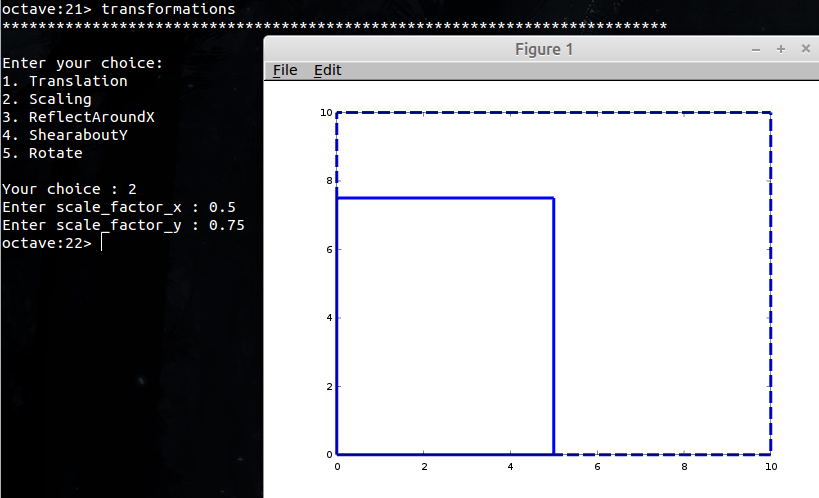
\includegraphics[width=60mm, height=60mm]{scalingMatlab.png}
\caption{scaling in Matlab\label{overflow}}
\end{figure}
\begin{figure}[ht!]
\centering
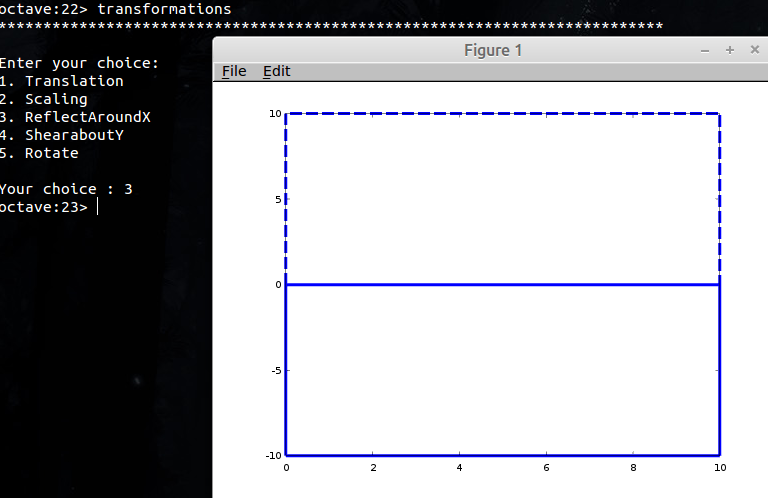
\includegraphics[width=60mm, height=60mm]{reflectionAboutXMatlab.png}
\caption{reflection in Matlab\label{overflow}}
\end{figure}
\begin{figure}[ht!]
\centering
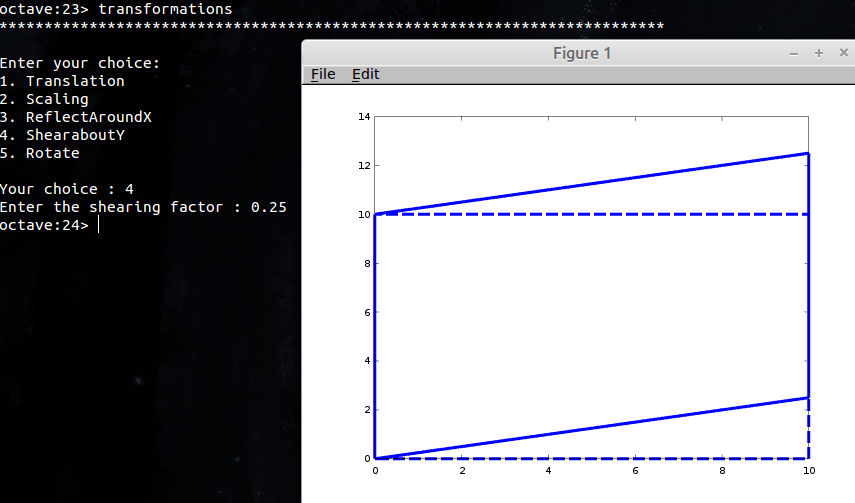
\includegraphics[width=60mm, height=60mm]{shearMatlab.png}
\caption{shear in Matlab \label{overflow}}
\end{figure}
\begin{figure}[ht!]
\centering
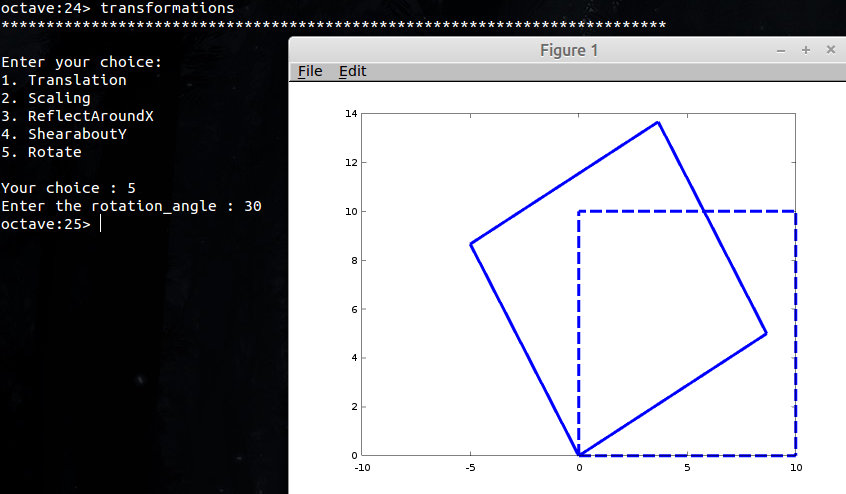
\includegraphics[width=60mm, height=60mm]{rotationMatlab.png}
\caption{Rotation in Matlab \label{overflow}}
\end{figure}
\end{document}
